
\documentclass[11pt,compress,t,notes=noshow,aspectratio=169,xcolor=table]{beamer}

\usepackage{../../style/lmu-lecture} % This file is included in slides and exercises

% Rarely used fontstyle for R packages, used only in 
% - forests/slides-forests-benchmark.tex
% - exercises/single-exercises/methods_l_1.Rnw
% - slides/cart/attic/slides_extra_trees.Rnw
\newcommand{\pkg}[1]{{\fontseries{b}\selectfont #1}}

% Spacing helpers, used often (mostly in exercises for \dlz)
\newcommand{\lz}{\vspace{0.5cm}} % vertical space (used often in slides)
\newcommand{\dlz}{\vspace{1cm}}  % double vertical space (used often in exercises, never in slides)
\newcommand{\oneliner}[1] % Oneliner for important statements, used e.g. in iml, algods
{\begin{block}{}\begin{center}\begin{Large}#1\end{Large}\end{center}\end{block}}

% Don't know if this is used or needed, remove?
% textcolor that works in mathmode
% https://tex.stackexchange.com/a/261480
% Used e.g. in forests/slides-forests-bagging.tex
% [...] \textcolor{blue}{\tfrac{1}{M}\sum^M_{m} [...]
% \makeatletter
% \renewcommand*{\@textcolor}[3]{%
%   \protect\leavevmode
%   \begingroup
%     \color#1{#2}#3%
%   \endgroup
% }
% \makeatother


\tikzset{main node/.style={rectangle,draw,minimum size=1cm,inner sep=4pt}}

\title{Interpretable Machine Learning} \date{}

\newcommand{\titlefigure}{figure/ebm.jpg} \newcommand{\learninggoals}{ \item Motivation from GAM \item Intelligible GAM \item Accurate GAM + Pairwise Interactions \item FAST feature interaction detection }

\lecturechapter{Explainable Boosting Machines} \lecture{Interpretable Machine Learning}

\begin{document}

\begin{frame}{Generalized Additive Models (GAMs)} \textbf{Recall the idea of GAMs:} \begin{equation*} g(\mathbb{E}(y_i \mid \mathbf{x}i)) = \theta_0 + \sum{j=1}^p f_j(x_{ij}) \end{equation*} \begin{itemize} \item Each $f_j$ captures the effect of a single feature \item Allows non-linear modeling of features, e.g. splines \item Interpretable as effects can be visualized individually \item Improves over GLMs by modeling non-linearity \item \textbf{Explainable Boosting Machines (EBMs)}: combine GAM structure with gradient boosting using small decision trees \citebutton{Lou et al. 2012}{https://www.cs.cornell.edu/~yinlou/papers/lou-kdd12.pdf} \end{itemize} \end{frame}

\begin{frame}{EBM: Boosting Intelligible GAMs - Initialization} \begin{itemize} \item Set all shape functions $f_j^{(0)} = 0$ \item Compute pseudo-residuals for all data points: \begin{itemize} \item For squared error: $r_i^{(0)} = y_i - \sum_j f_j^{(0)}(x_{ij})$ \item For log loss: $r_i^{(0)} = y_i - \sigma(\hat{y}_i^{(0)})$ where $\sigma$ is the sigmoid function \end{itemize} \item Begin sequential updates for each feature \end{itemize} 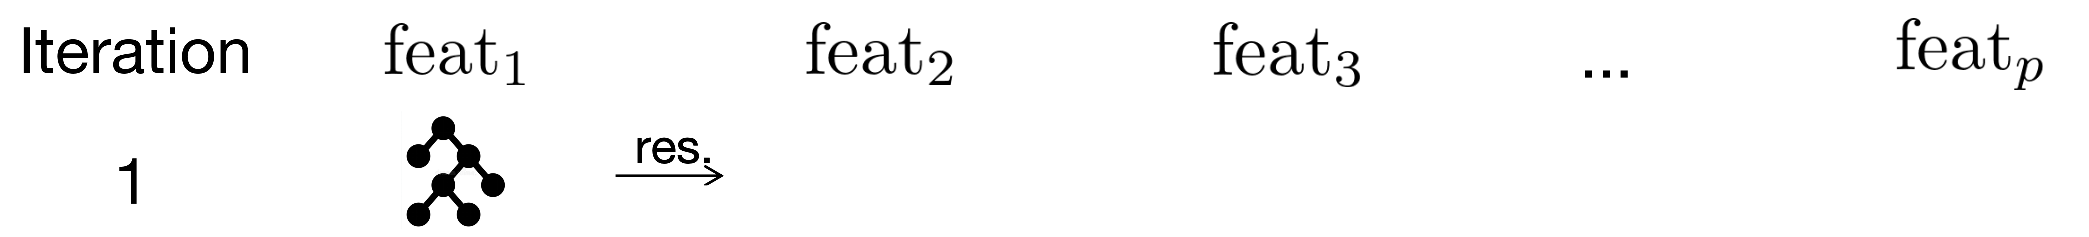
\includegraphics[width=1\linewidth]{figure/EBM_Step1.png} \end{frame}

\begin{frame}{EBM: Step-by-Step Boosting - Feature 1} \begin{itemize} \item Fit shallow tree $S_1^{(1)}$ to $(x_{i1}, r_i)$ \item Update $f_1^{(1)}(x_{i1}) = f_1^{(0)} + \eta \cdot S_1^{(1)}(x_{i1})$ \item Update prediction $\hat{y}i = \sum_j f_j(x{ij})$ \item Update residuals: $r_i^{(1)} = y_i - \hat{y}_i$ \item Move to next feature \end{itemize} 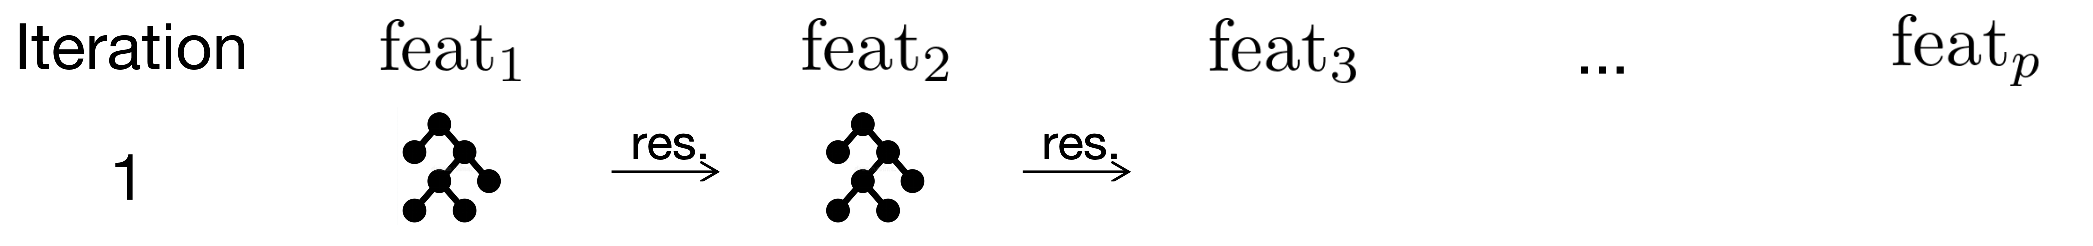
\includegraphics[width=1\linewidth]{figure/EBM_Step2.png} \end{frame}

\begin{frame}{EBM: Sequential Feature Updates} \begin{itemize} \item Repeat boosting steps sequentially over all features \item Each update uses shallow trees (2--4 leaves) to prevent overfitting \item Continue for $M$ iterations \item Use small learning rate $\eta$ so feature order doesn't matter \end{itemize} 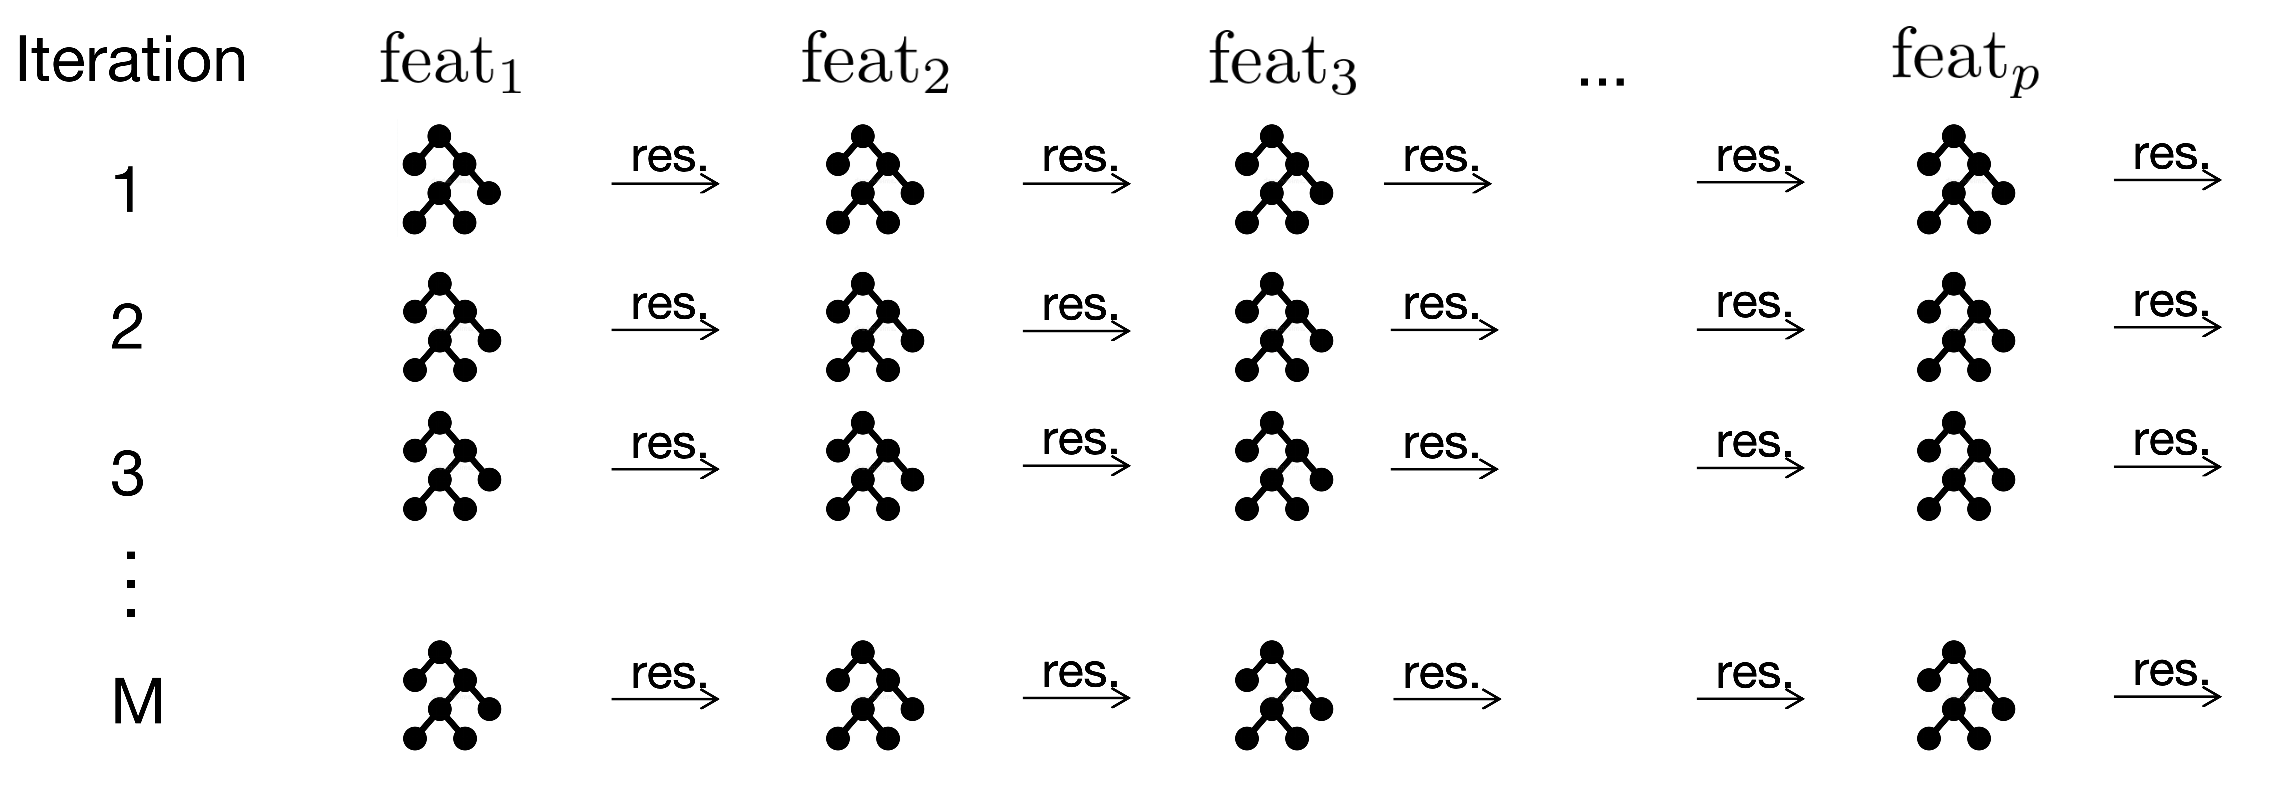
\includegraphics[width=1\linewidth]{figure/EBM_Step3.png} \end{frame}

\begin{frame}{EBM: Prediction and Interpretation} \begin{itemize} \item $f_j(x_j) = \sum_{m=1}^{M} \eta S_j^{(m)}(x_j)$ for each $j$ \item Final model: $\hat{y} = \theta_0 + \sum_j f_j(x_j)$ \item Each $f_j$ visualized as a 2D plot: $x_j$ vs. $f_j(x_j)$ \item 2D plots provide transparent interpretation of marginal effects \end{itemize} 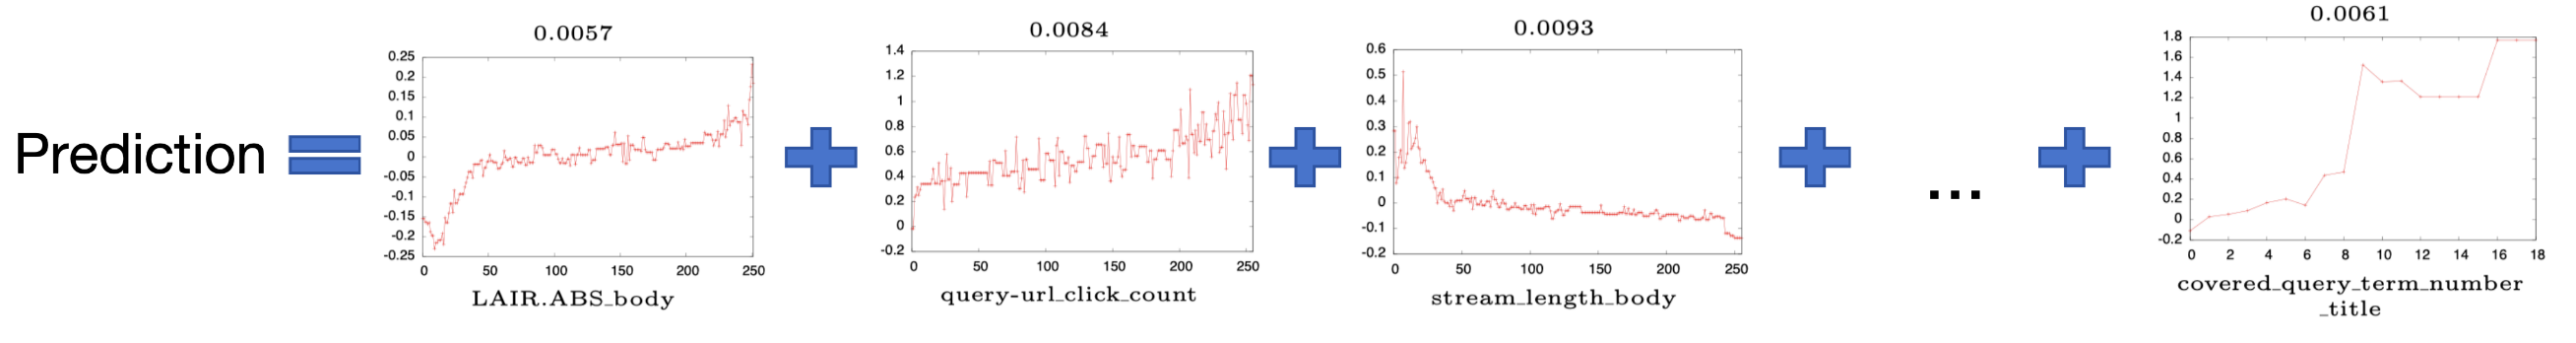
\includegraphics[width=1.3\linewidth]{figure/ebm_prediction.png} \end{frame}

\begin{frame}{EBM: Advantages and Extensions} \begin{itemize} \item Shallow bagged trees per feature yield discrete, robust shape functions \item Low variance, interpretable \item Limitations: can't model interactions between features \item Next step: Add selected pairwise interaction terms using \textbf{FAST} algorithm \citebutton{Lou et al. 2013}{https://www.cs.cornell.edu/~yinlou/papers/lou-kdd13.pdf} \end{itemize} \end{frame}

\begin{frame}{Generalized Additive Models + Interactions} \begin{equation*} g(\mathbb{E}(y \mid \xv)) = \theta_0 + \sum_i f_i(x_i) + \sum_{i<j} f_{ij}(x_i, x_j) \end{equation*} \begin{itemize} \item Enables modeling of 2D interactions while preserving intelligibility \item $O(p^2)$ potential terms \textemdash{} must select top $K$ \item Interaction strength estimated via residual sum of squares (RSS) reduction \item \textbf{FAST algorithm}: efficiently ranks pairs without building full models \end{itemize} \end{frame}

\begin{frame}{FAST Algorithm: Tree-Like Interaction Modeling} \begin{columns}[T, totalwidth=\textwidth] \begin{column}{0.5\textwidth} 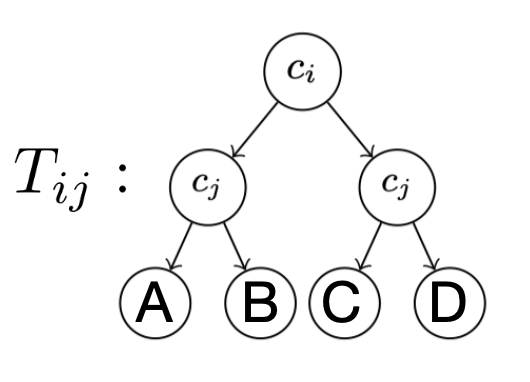
\includegraphics[width=0.6\linewidth]{figure/T_ij.png} 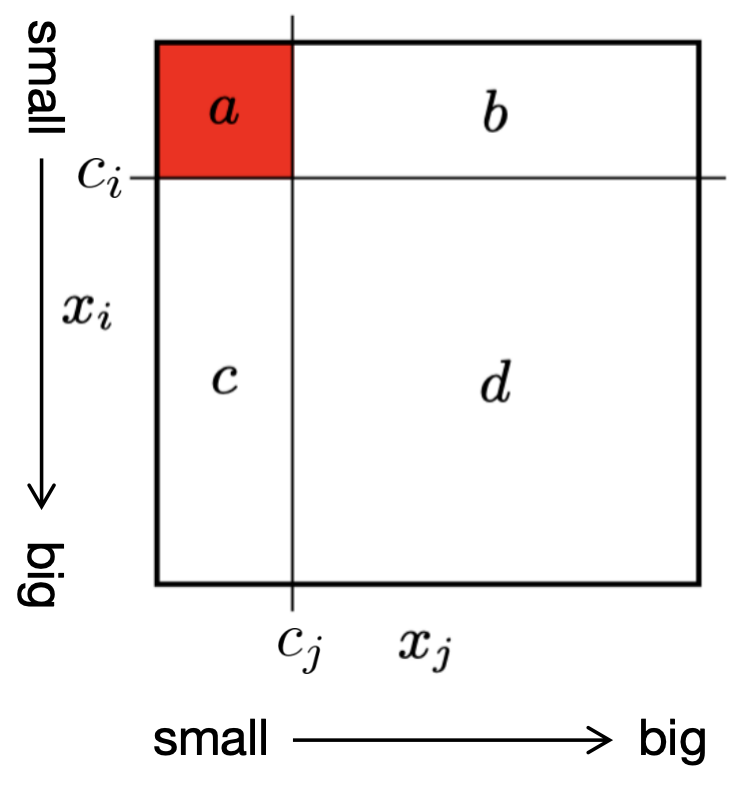
\includegraphics[width=0.65\linewidth]{figure/FAST1.png} \end{column} \begin{column}{0.5\textwidth} \begin{itemize} \item $T_{ij}$: 4-leaf tree with cut points $c_i, c_j$ on features $x_i$, $x_j$ \item Each region $r \in {A,B,C,D}$: predict with mean target value in region \item Calculate RSS from predictions: $\text{RSS}{ij} = \sum_k (y_k - T{ij}(x_k))^2$ \item Optimize cutpoints $(c_i, c_j)$ to minimize $\text{RSS}_{ij}$ \end{itemize} \end{column} \end{columns} \end{frame}

\begin{frame}{FAST: Dynamic Programming with Cumulative Histograms} \begin{itemize} \item Compute cumulative target sums $CH_j^t(c_j)$ and counts $CH_j^w(c_j)$ \item Build lookup tables $L^t(c_i, c_j)$ and $L^w(c_i, c_j)$ for targets and weights \item For each $(c_i, c_j)$, derive $\hat{y}_r = \text{sum}/\text{count}$ in each region \item Estimate RSS efficiently from table values without recomputation \end{itemize} 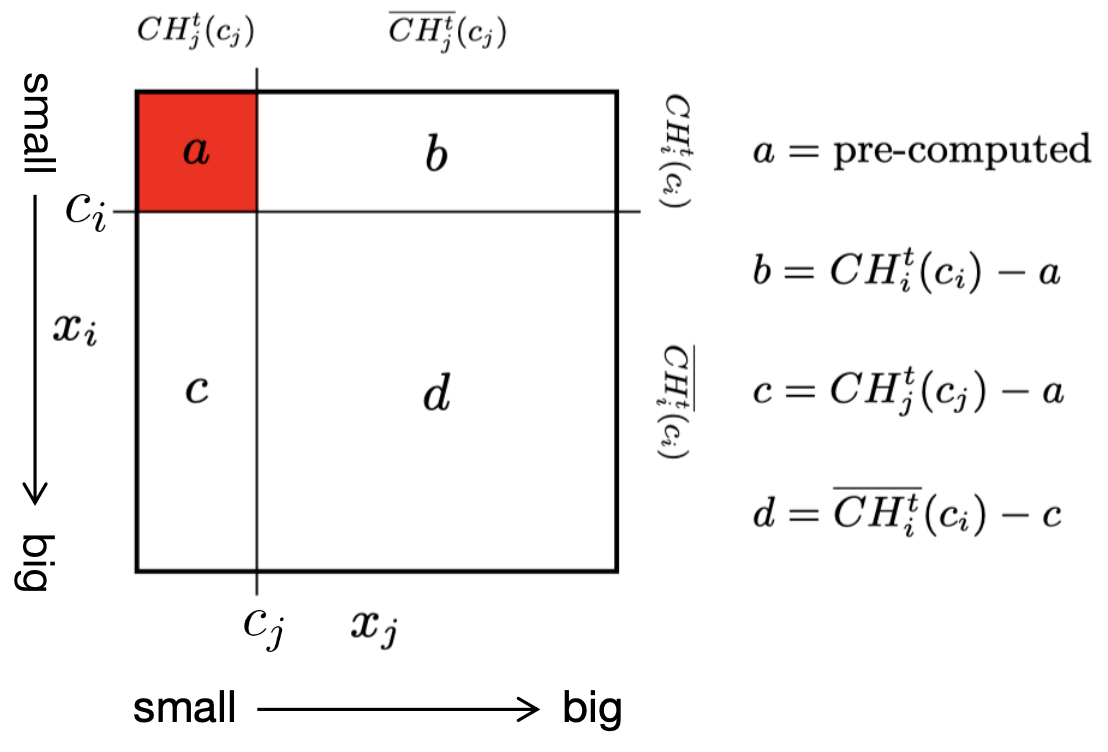
\includegraphics[width=\linewidth]{figure/FAST.png} \end{frame}

\begin{frame}{FAST: Final Ranking of Interactions} \begin{itemize} \item For discretized features with $d_i, d_j$ values: $d_id_j$ possible $(c_i,c_j)$ combinations \item For each: compute $\text{RSS}_{ij}$ and store best value \item Assign interaction strength as max RSS reduction for the pair \item Rank all $\binom{p}{2}$ pairs, select top $K$ \end{itemize} \end{frame}

\begin{frame}{GA2M: Two-Stage Model Construction} \begin{enumerate} \item Train EBM with $p$ univariate shape functions $f_j$ \item Compute residuals and use FAST to rank pairwise interactions \item Select $K$ top interactions $f_{ij}(x_i, x_j)$ \item Train additive model combining $f_j$ and $f_{ij}$ \end{enumerate} \end{frame}

\begin{frame}{GA2M: Visualization and Prediction} \begin{itemize} \item Retain 2D plots for $f_j$, add 3D heatmaps for $f_{ij}$ \item Predict $\hat{y} = \theta_0 + \sum_j f_j(x_j) + \sum_{(i,j)\in K} f_{ij}(x_i, x_j)$ \item Each model component interpretable independently \end{itemize} 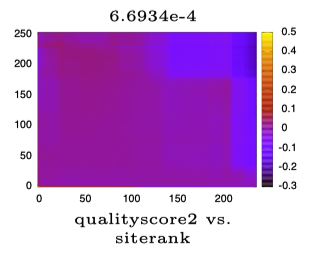
\includegraphics[width=0.5\linewidth]{figure/3D Heatmap.png} \end{frame}

\begin{frame}{EBM-GA2M: Summary} \begin{itemize} \item EBMs extend GAMs via boosting of low-depth trees \item FAST enables tractable interaction detection \item GA2M = EBM + selected pairwise functions \item Near full-complexity accuracy with visual transparency \end{itemize} 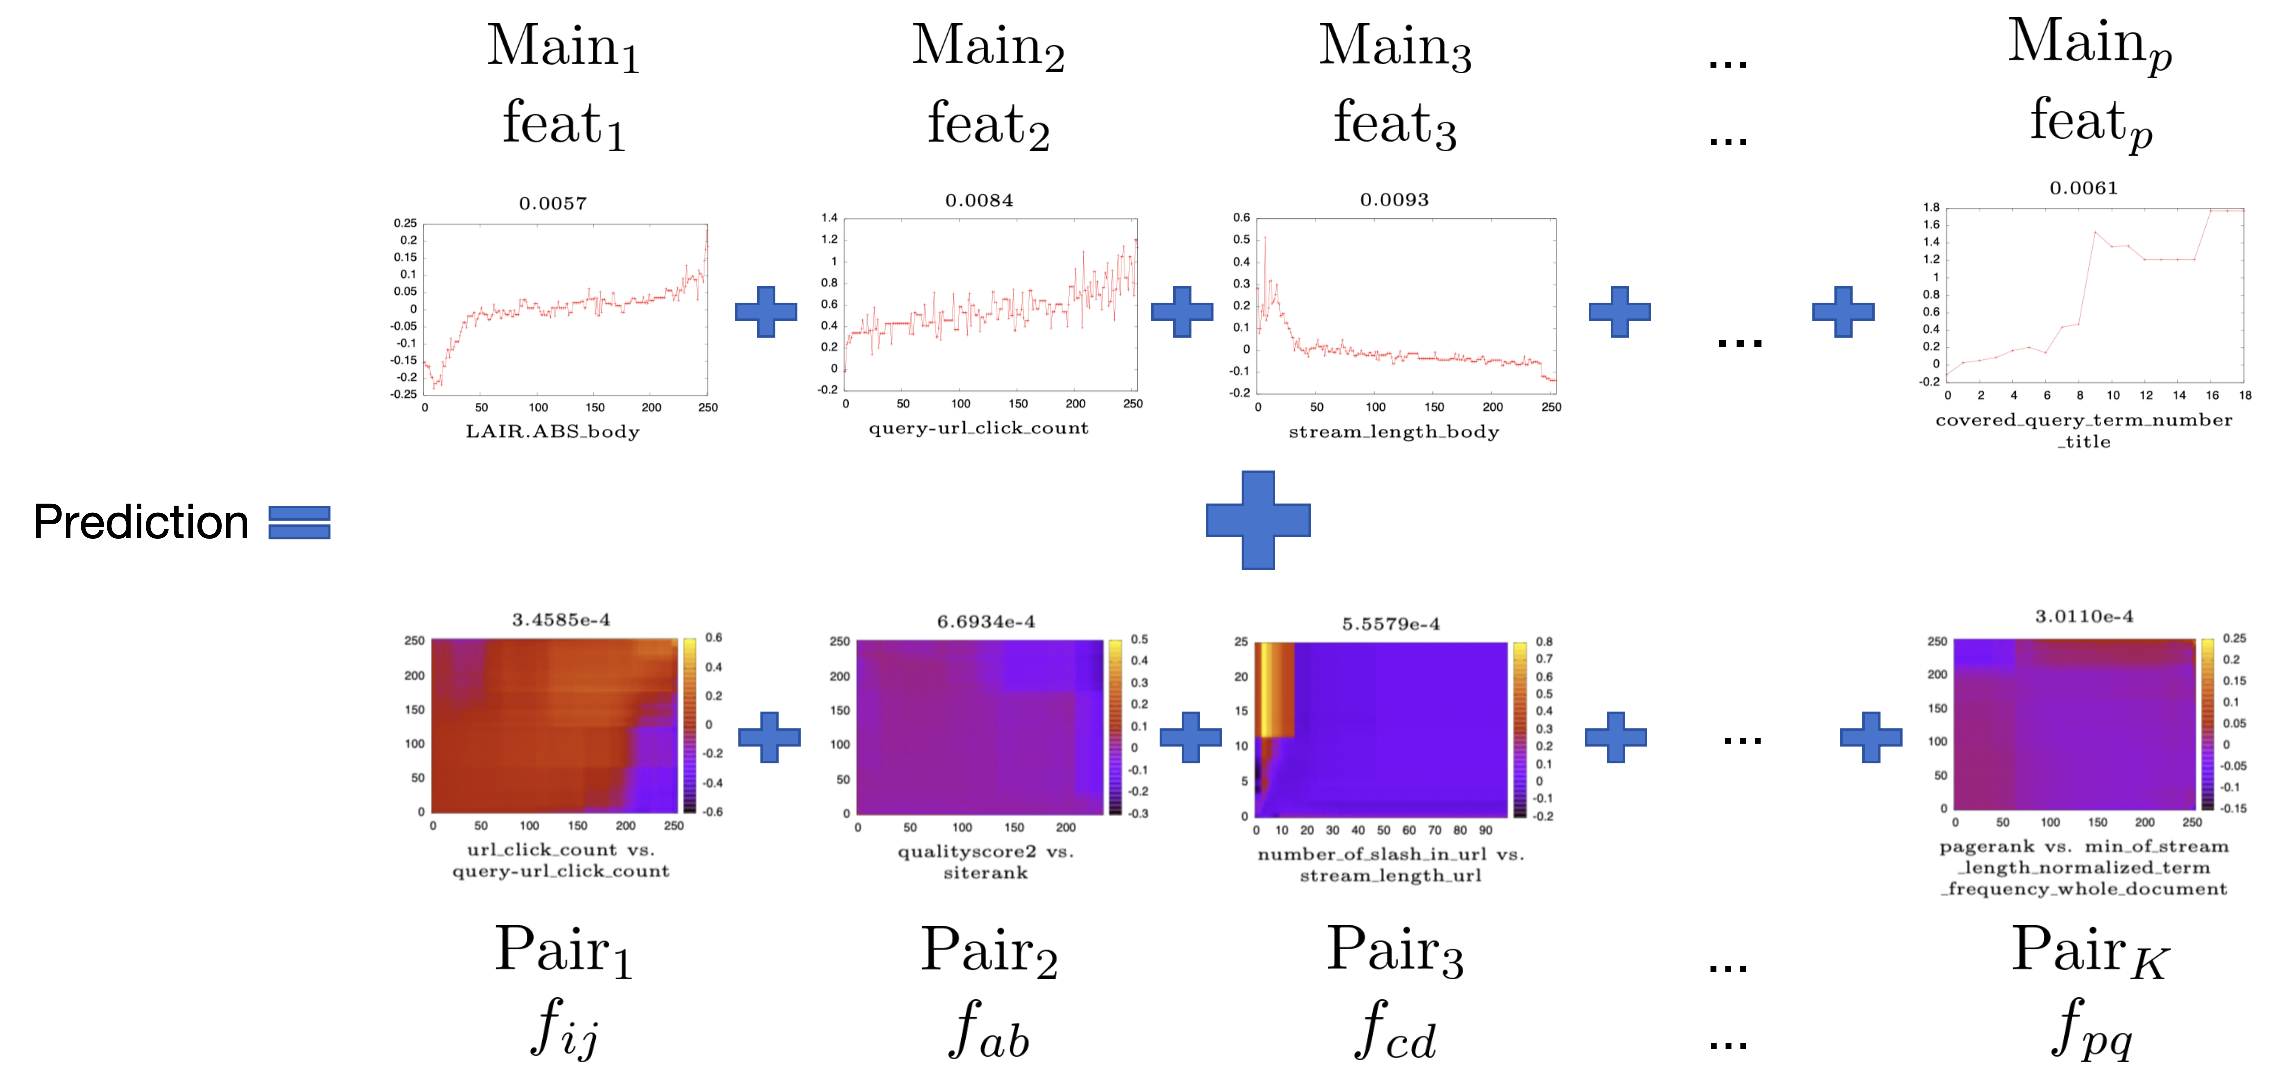
\includegraphics[width=1\linewidth]{figure/final_ebm.png} \end{frame}

\end{document} 

